% Variance partition of the model-discrepancy budget on b = beta - 1.
% The slice idiom is justified here because the quantity really is a
% partition: sigma_model^2 is the sum of the squared terms.
% Compile from `docs/preprint`:  lualatex sekil/paylar.tex
\documentclass[border=3pt,tikz]{standalone}
\usepackage{amsmath}
\usepackage{bm}
\usepackage[outline]{contour}
\usetikzlibrary{calc,shadows.blur,arrows.meta}
\contourlength{0.3pt}
\tikzset{>=latex}

\colorlet{ink}{black!82}
\colorlet{missing}{red!72!black}
\colorlet{site}{orange!85!black}
\colorlet{plateau}{blue!55!cyan!75!black}
\colorlet{realis}{violet!60!black}
\colorlet{shape}{teal!60!black}
\colorlet{farres}{black!50}

\def\R{2.5}
\tikzset{slice/.style={fill=#1, draw=#1!75!black, line join=round,
  line width=0.4, blur shadow={shadow blur steps=18, shadow xshift=0.4,
  shadow yshift=-0.8, shadow opacity=30}},
  lead/.style={draw=#1, line width=0.35pt, shorten >=1.5pt}}

\begin{document}
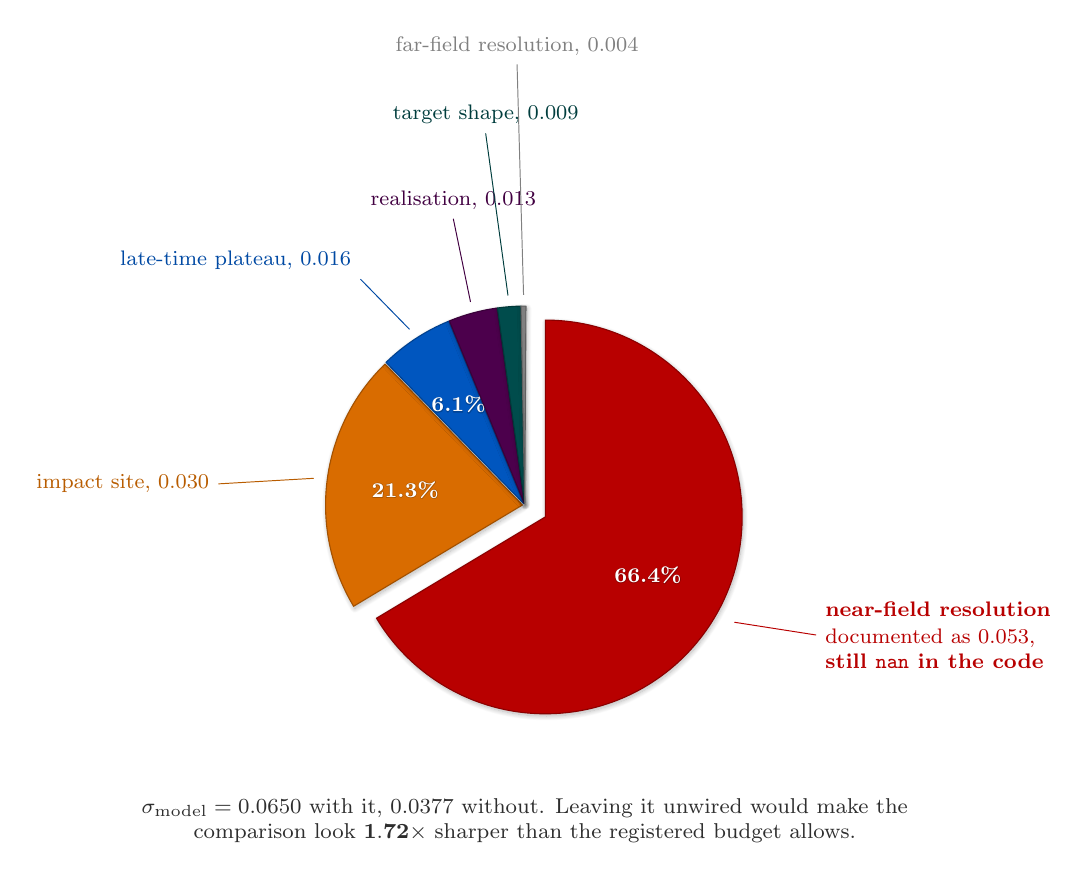
\begin{tikzpicture}[font=\footnotesize]

% Slices run clockwise from 90 degrees. The mid-angles below are the ones
% the leader lines point at; an earlier version placed them by hand and
% they pointed at the wrong wedges.
\foreach \frac/\col/\exp [
    remember=\angb as \anga (initially 90),
    evaluate={\angm=\anga-\frac*1.8;
              \angb=\anga-\frac*3.6;
              \rr=\exp+\R*0.60;}
  ] in {%
    66.4/missing/0.30,
    21.3/site/0.03,
     6.1/plateau/0.03,
     4.0/realis/0.03,
     1.9/shape/0.03,
     0.4/farres/0.03%
  }{
    \draw[slice=\col] (\angm:\exp) --++ (\anga:\R)
          arc(\anga:\angb:\R) -- cycle;
    \ifdim \frac pt > 5pt
      \node[white, scale=0.95] at (\angm:\rr)
        {\contour{\col!78!black}{\bm{$\frac\mathbf{\%}$}}};
    \fi
  }

% --- labels, anchored on the true mid-angles ---------------------------
\node[text=missing, anchor=west, align=left, scale=0.95] (lm) at (-24:4.05)
     {\textbf{near-field resolution}\\[1pt]
      documented as $0.053$,\\
      \textbf{still \texttt{nan} in the code}};
\draw[lead=missing] (lm.west) -- (-29.5:3.0);

\node[text=site!85!black, anchor=east, scale=0.95] (ls) at (176:3.9)
     {impact site, $0.030$};
\draw[lead=site!85!black] (ls.east) -- (172.5:2.65);

\node[text=plateau!85!black, anchor=south east, scale=0.95] (lp) at (126:3.55)
     {late-time plateau, $0.016$};
\draw[lead=plateau!85!black] (lp.south east) -- (123:2.62);

\node[text=realis!85!black, anchor=south, scale=0.95] (lr) at (104:3.75)
     {realisation, $0.013$};
\draw[lead=realis!85!black] (lr.south) -- (105:2.62);

\node[text=shape!80!black, anchor=south, scale=0.95] (lh) at (96:4.75)
     {target shape, $0.009$};
\draw[lead=shape!80!black] (lh.south) -- (94.5:2.62);

\node[text=farres, anchor=south, scale=0.95] (lf) at (91:5.6)
     {far-field resolution, $0.004$};
\draw[lead=farres] (lf.south) -- (90.3:2.62);

% --- the consequence ----------------------------------------------------
\node[ink, anchor=north, align=center, scale=0.97] at (0,-3.6)
  {$\sigma_{\rm model}=0.0650$ with it, $0.0377$ without.
   Leaving it unwired would make the\\comparison look
   $\mathbf{1.72\times}$ sharper than the registered budget allows.};

\end{tikzpicture}
\end{document}
